The same three tasks are added in the blackboard with unique altitudes for easy differentation. To start a team architecture,
start the script \textit{2\_TeamController.sh}. This will, again, start n \acp{uav} (previously passed as parameter when starting the containers).
Only now, each \acs{uav} is added to a team. Each team has its own goal to complete. For example team 1 has the goal to complete task A and will
only complete this task.

In this example 7 \acp{uav} are split up into three teams of size three with the last team only container one \acs{uav}.

\begin{figure}[ht]
    \centering
    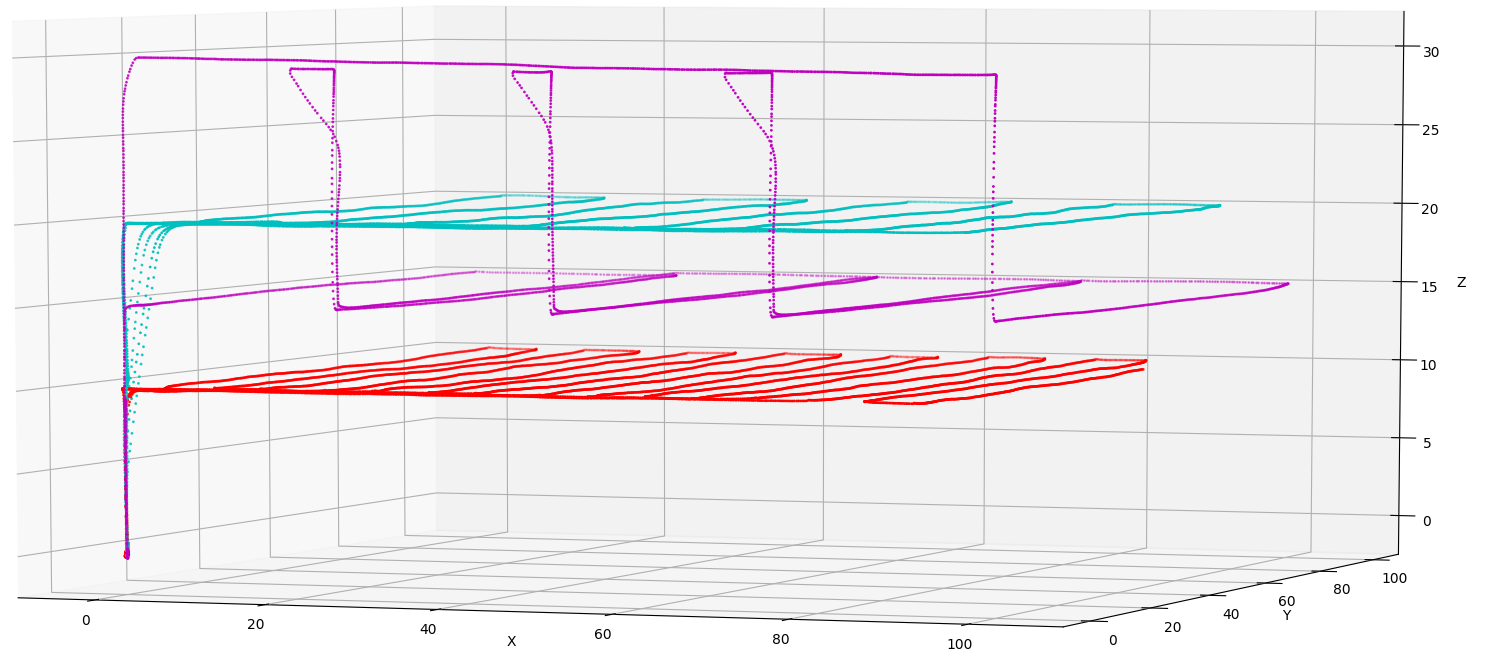
\includegraphics[scale=0.3]{teams_size_3/team7Full.png}
    \caption[teams architecture]{teams flight patters}
\end{figure}

Each team has its unique color. In the figure it becomes clear that each team completed a task. 

\newpage
\begin{figure}[ht]
    \centering
    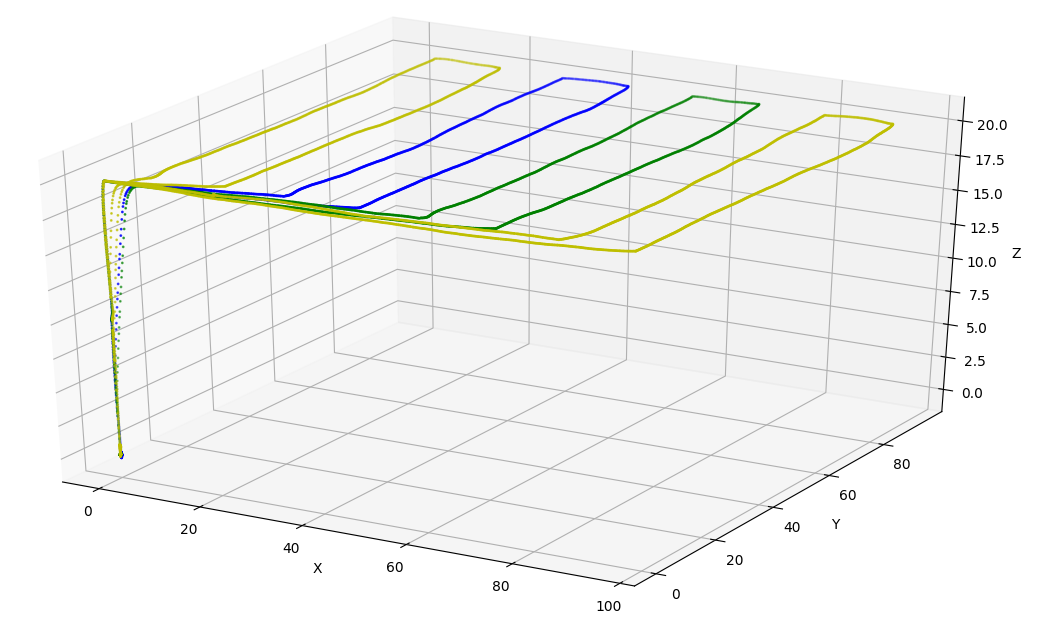
\includegraphics[scale=0.3]{teams_size_3/team2_unique.png}
    \caption[teams architecture]{teams flight patters}
\end{figure}

Analyzing the flights patterns of a single team clarifies that each drone in the team completed at least one task.

\begin{figure}[ht]
    \centering
    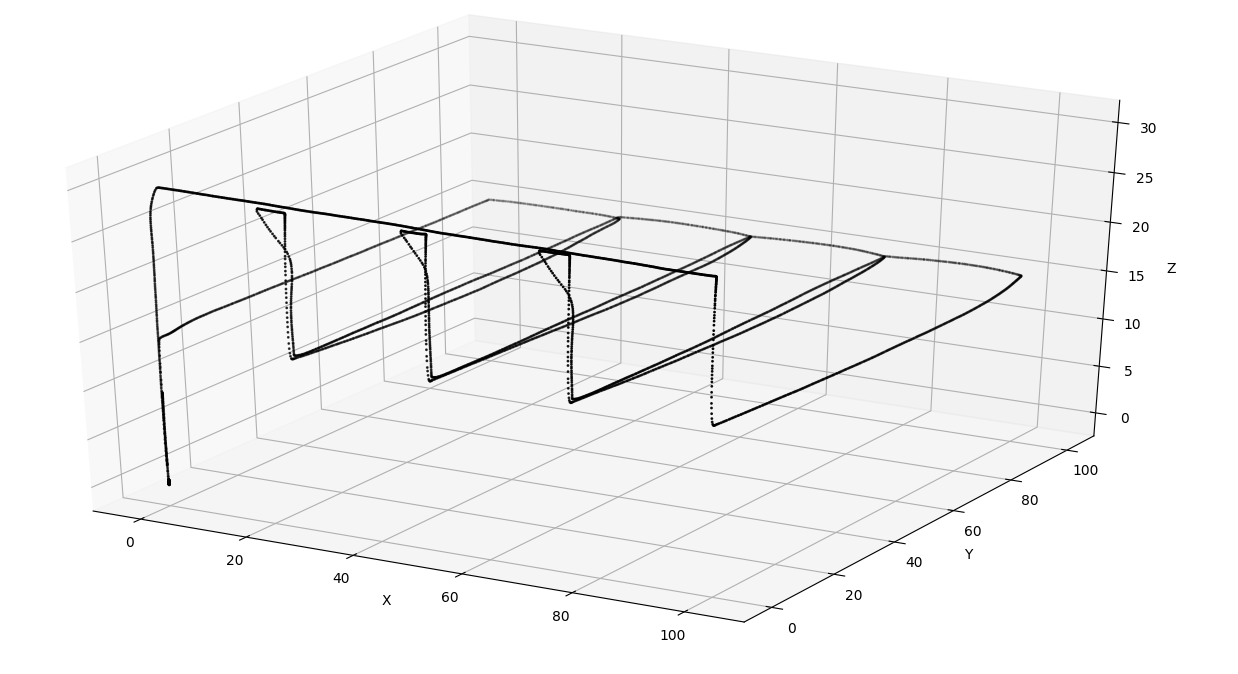
\includegraphics[scale=0.3]{teams_size_3/team3_unique.png}
    \caption[teams architecture]{teams flight patters}
\end{figure}

Even in the last team, only containing one \acs{uav}, completed all its tasks.